
\title{T-61.5130 Machine Learning and Neural Networks}
\author{Karhunen, Luttinen}
\date{Exercise 9, 30.11.2012}

\usepackage{pdfpages}

\usepackage{subfig}


\newcommand{\vect}[1]{{\bf{#1}}}
\newcommand{\svect}[1]{\boldsymbol{#1}}
\newcommand{\matr}[1]{\boldsymbol{#1}}

\renewcommand{\vec}[1]{\mathbf{#1}}
\newcommand{\set}[1]{\mathcal{#1}}
\newcommand{\C}{\set{C}}
\newcommand{\E}{\mathcal{E}}
\newcommand{\I}{\vec{I}}
\renewcommand{\L}{\mathcal{L}}
\newcommand{\N}{\mathrm{I \negmedspace N}}
\newcommand{\R}{\mathrm{I \negmedspace R}}
\newcommand{\V}{\set{V}}
\newcommand{\W}{\vec{W}}
\newcommand{\X}{\set{X}}
\newcommand{\e}{\vec{e}}
% \newcommand{\f}[1]{\mathrm{#1}} %funktio
\newcommand{\h}{\vec{h}}
\newcommand{\m}{\vec{m}}
\newcommand{\mub}{\boldsymbol{\mu}}
\newcommand{\n}{\vec{n}}
\renewcommand{\t}{\vec{t}}
\renewcommand{\u}{\vec{u}}
\renewcommand{\v}{\vec{v}}
\newcommand{\w}{\vec{w}}
\newcommand{\x}{\vec{x}}
\newcommand{\y}{\vec{y}}
\newcommand{\Y}{\vec{Y}}
\newcommand{\z}{\vec{z}}
\newcommand{\argmin}{\operatornamewithlimits{argmin}}
\newcommand{\argmax}{\operatornamewithlimits{argmax}}
\newcommand{\bSigma}{\boldsymbol{\Sigma}}



\begin{document}

\maketitle

\begin{enumerate}

\item Consider a random input vector $\mathbf{X}$ made up of two component vectors,
  $\mathbf{X} = [\mathbf{X}_1,\mathbf{X}_2]^T$. Assume that you would like to represent the
  central dependencies between $\mathbf{X}_1$ and $\mathbf{X}_2$ with a  simple
  model. How would you do that? (Hint: Consider linear combinations.)

  \begin{solution}

    If we are not interested in the dependencies inside the groups
    $\vec{X}_1$ or $\vec{X}_2$ but are interested only on dependecies
    between these groups, we can use canonical correlation analysis
    (CCA).  It means that we try to find projections from $\vec{X}_1$
    and $\vec{X}_2$ which would be as correlated as possible. CCA uses
    only second-order statistics; for Gaussian variables this is
    sufficient but CCA can also be used for non-Gaussian
    variables. For a tutorial on CCA, see, e.g., the one by Magnus
    Borga available at http://people.imt.liu.se/$\sim$magnus/cca/
    . The following is partly based on the information in that
    tutorial.

    The correlation coefficient between zero mean random variables $a$
    and $b$ is defined to be $\rho_{ab} =
    E\{ab\}/\sqrt{E\{a^2\}E\{b^2\}}$.  We have projections $a_i =
    \u_i^T \x_1$ and $b_i = \v_i^T \x_2$ and we would like to maximise
    the correlations between $a_i$ and $b_i$. We restrict the
    solutions to be uncorrelated for different $i$.
    % Thus, the task
    % is:
    % \begin{align*}
    %   \text{maximize:} &\quad \rho_{ab} = \frac{E\{ab\}}
    %   {\sqrt{E\{a^2\}E\{b^2\}}}
    %   \\
    %   \text{subject to:} &\quad E\{a_i a_j\} = E\{b_i b_j\} = E\{a_i
    %   b_j\} = 0, \quad \forall i \neq j
    % \end{align*}
    
    % For the $i$th projections we have
    % \begin{align*}\nonumber
    %   \rho_{a_i b_i}
    %   = \frac{E\{\u_i^T \x_1 \x_2^T \v_i\}}{\sqrt{E\{\u_i^T \x_1\x_1^T\u_i\} E\{\v_i^T \x_2\x_2^T\v_i\}}}
    %   &= \frac{\u_i^T E\{\x_1 \x_2^T\} \v_i}{\sqrt{\u_i^T E\{\x_1\x_1^T\}\u_i \v_i^T E\{\x_2\x_2^T\}\v_i}} \\
    %   &= \frac{\u_i^T \boldsymbol{\Sigma}_{12} \v_i}{\sqrt{\u_i^T \boldsymbol{\Sigma}_1\u_i \v_i^T \boldsymbol{\Sigma}_2\v_i}} \;.
    % \end{align*}

    % It can be shown that the maximization corresponds to solving either one
    % of the following eigenvalue equations:
    % $$
    % \bSigma_1^{-1}\bSigma_{12}\bSigma_2^{-1}\bSigma_{12}^T\u_i=\rho^2_{a_i b_i}\u_i
    % $$
    % $$
    % \bSigma_2^{-1}\bSigma_{12}^T\bSigma_1^{-1}\bSigma_{12}\v_i=\rho^2_{a_i b_i}\v_i \;.
    % $$


    % \paragraph{Connection to singular value decomposition.}
    
    Canonical correlations are invariant to affine transformations
    (for example, if a transformation $\mathbf{A}$ is used for $\x_1$,
    just set $\hat \u_i=\mathbf{A}^{-1}\u_i$).  Therefore, to simplify
    the situation, suppose that $\vec{X}_1$ and $\vec{X}_2$ have been
    whitened.
    %(see problem 3 for the precise transformations needed).
    Then $\bSigma_1=\mathbf{I}$ and $\bSigma_2=\mathbf{I}$.
    \begin{align*}
      \mathrm{cov}\left\{
        \begin{bmatrix}
          \mathbf{x}_1
          \\
          \mathbf{x}_2
        \end{bmatrix}
      \right\}
      =
      \begin{bmatrix}
        \mathbf{I} & \mathbf{\Sigma}_{12}
        \\
        \mathbf{\Sigma}_{21} & \mathbf{I}.
      \end{bmatrix}
    \end{align*}
    (Note that $\vec{X}_1$ and $\vec{X}_2$ can have different
    dimensionalities, so the two identity matrices can be of different
    sizes.)
    % The eigenvalue equations then become
    % \begin{equation}\label{eq:temp1}
    %   \bSigma_{12}\bSigma_{12}^T\u_i=\rho^2_{a_i b_i}\u_i\;,\;
    %   \bSigma_{12}^T\bSigma_{12}\v_i=\rho^2_{a_i b_i}\v_i \;.
    % \end{equation}
    % 
    Now, we want to maximize the correlation coefficient:
    \begin{align*}
      \rho_{a_i b_j} &= \frac{E\{a_i b_j\}} { \sqrt{ E\{a_i^2\}
          E\{b_j^2\} } }
      \\
      &= \frac{ \mathbf{u}_i^T \overbrace{E\{\mathbf{x}_1
          \mathbf{x}_2^T \}}^{\mathbf{\Sigma}_{12}} \mathbf{v}_j } {
        \sqrt{ \strut \mathbf{u}_i^T
          \smash{\underbrace{E\{\mathbf{x}_1
              \mathbf{x}_1^T\}}_{\mathbf{I}}} \mathbf{u}_i
          \mathbf{v}_i^T \smash{\underbrace{E\{\mathbf{x}_2
              \mathbf{x}_2^T\}}_{\mathbf{I}}} \mathbf{v}_i } }
      \\
      \\
      &= \frac{ \mathbf{u}_i^T} {\|\mathbf{u}_i\|}
      \mathbf{\Sigma}_{12} \frac{ \mathbf{v}_j } { \|\mathbf{v}_j\|}.
    \end{align*}
    From this it is obvious that the correlation is maximized when
    $\mathbf{u}_1$ and $\mathbf{v}_1$ are the left and right singular
    vectors corresponding to the largest singular value of
    $\mathbf{\Sigma}_{12}$.  In general, the remaining projections
    maximize correlation while satisfying the uncorrelation
    requirement if $\mathbf{u}_i$ and $\mathbf{v_i}$ are the left and
    right singular vectors corresponding to the $i$-th largest
    singular value of $\mathbf{\Sigma}_{12}$.

    See exercise session 3 for more information about the
    \emph{singular value decomposition} (SVD).
  \end{solution}
  
\item Show that
  \begin{displaymath}
    I(X;Y) = D\left( p(X,Y) \| p(X)p(Y) \right) ,
  \end{displaymath}
  that is, mutual information is equal to the Kullback-Leibler
  divergence of the joint distribution from the ``corresponding''
  factored distribution.

  \begin{solution}

    Starting from the definition $I(X; Y) = h(X) - h(X | Y)$, where $h(X)$
    is
    \[
    h(X) = -\int_{-\infty}^{\infty} f_X(x) \log f_X(x)dx = -E[\log f_X(x)]
    \] 
    and $h(X|Y)$ is
    \[
    h(X|Y)=-\int_{\infty}^{\infty}\int_{\infty}^{\infty}f_{X,Y}(x,y)\log
    f_X(x|y) dx dy
    \]
    we have
    \begin{equation}
      \begin{split}
        I(X; Y) &= -\int p(x) \ln p(x) dx + \int p(x, y) \ln p(x | y) dx dy\\ 
        &= -\int p(x, y) \ln p(x) dx dy + \int p(x, y) \ln \frac{p(x, y)}{p(y)} dx dy\\ 
        &= \int p(x, y) \ln \frac{p(x, y)}{p(x) p(y)} dx dy \\
        &= D\left(p(x, y) \| p(x)p(y)\right)
      \end{split}
    \end{equation}


  \end{solution}

  
\item Show that for a transformation $\mathbf{y} = \mathbf{W}
  \mathbf{x}$ there exists a simple connection between mutual information $I$
  and negentropy $J$ assuming that the $Y_i$ are uncorrelated and have
  unit variance:
  \[
  I(Y_1, \ldots , Y_n) = C - \sum_{i=1}^n J(Y_i) ; ,
  \]
  where $C$ is a constant. (Notation: $y_i$ is the value of the random
  variable $Y_i$.) What does this connection imply for ICA computation?

  \begin{solution}

    Negentropy measures how much the (differential) entropy of a distribution
    differs from that of the Gaussian distribution having the same
    variance.  If $h_G(Y_i)$ denotes the entropy of the Gaussian
    distribution having the same variance as the random variable $Y_i$,
    the negentropy is
    \begin{align*}
      J(Y_i) = h_G(Y_i) - h(Y_i) \quad (\geq 0).
    \end{align*}
    Recall that from all distributions with a given variance, the
    Gaussian distribution has the highest entropy.  Negentropy is thus
    always non-negative and is zero if and only if $Y_i$ has a
    Gaussian distribution.

    The mutual information can be written as
    \begin{align*}
      I(Y_1, \ldots, Y_n) &= \sum_{i=1}^n h(Y_i) - h(Y_1, \ldots, Y_n)
      \\
      &= \sum_{i=1}^n [\underbrace{h_G(Y_i)}_{\text{constant}} - J(Y_i)] - h(Y_1, \ldots, Y_n)
      % = C -
      % \sum_{i=1}^n J(Y_i) ,
    \end{align*}
    %where $C$ is constant.
    The terms $h_G(Y_i)$ are clearly constant since the variance for
    all $Y_i$ was defined to be the same (unity) and the entropy of a
    Gaussian scalar variable depends only on its variance.

    $Y$ is defined to have a unit covariance matrix; this means that
    different transformation matrices ${\bf W}$ can differ only by an
    orthogonal rotation.
    %
    % In fact, if ${\bf C}_X$ is the covariance matrix of the
    % observations $X$, then a unit covariance for $Y$ implies  
    % \begin{equation*}
    %   {\bf W} {\bf C}_X {\bf W}^T =  { \bf W} {\bf C}_X^{1/2} ( {\bf W} {\bf C}_X^{1/2} )^T =
    %   {\bf I}  
    % \end{equation*}
    % meaning that ${\bf U} = { \bf W} {\bf C}_X^{1/2}$ is an orthonormal matrix and
    % ${ \bf W} = {\bf U} {\bf C}_X^{-1/2}$.
    %
    % In fact,
    % \begin{align*}
    %   E[ \mathbf{W}  ]  
    % \end{align*}
    % (see the solution to exercise problem
    % 6.1). 
    %
    % The term $h(Y_1, \ldots, Y_n)$ is constant because
    % entropy does not change in translations or orthogonal rotations;
    % this is because they leave the form of the probability density
    % untouched. 
    The term $h(Y_1, \ldots, Y_n)$ is not changed by translations or
    orthogonal rotations because if $\mathbf{z}=\mathbf{Ry}$, where
    $\mathbf{R}$ is an orthogonal matrix, we have:
    \begin{align*}
      p_Z(\mathbf{z}) = p_Y(\mathbf{y})
      \underbrace{|\det{\mathbf{R}}|^{-1}}_{=1} = p_Y(\mathbf{y}).
    \end{align*}
    Thus, $h(Y)$ is constant with respect to orthogonal rotations of
    $Y$.  Therefore, $h(Y_1, \ldots, Y_n)$ is constant with respect to
    $\mathbf{W}$ under the whitening constraint.  Thus,
    \begin{align*}
      I(Y_1, \ldots, Y_n) = \sum_{i=1}^n
      [\underbrace{h_G(Y_i)}_{\text{constant}} - J(Y_i)] -
      \underbrace{h(Y_1, \ldots, Y_n)}_{\text{constant}} = C -
      \sum_{i=1}^n J(Y_i).
    \end{align*}
    % Thus any choice ${ \bf W}$ gives the same joint entropy as
    % projecting with ${\bf C}_X^{-1/2}$
    % and minimizing $I(Y_1, \ldots, Y_n)$ amounts to maximizing the
    % sum of negentropies.

    ICA can be defined as the search for the rotation which minimises
    the mutual information between the resulting components.  The above
    discussion shows that this can be done also by
    maximising the negentropies of the components.

  \end{solution}
  
\item How to reduce noise in natural images using ICA?

  % Is it really useful to teach image denoising with ICA? I think ICA
  % is better understood as an explorative tool, where you'll extract
  % interesting independent components from the data signals.

  \begin{solution}

    \begin{itemize}
    \item We have a set of $M$ images. Preprocess the images (zero
      mean and unit variance).  The images are assumed to be corrupted
      by isotropic Gaussian noise with variance $\sigma^2$.
    \item Choose randomly a training set of $N$ (e.g., $10000$) image
      patches (windows) of $D \times D$ (e.g., $16 \times 16$) pixels.
      Form $D^2 \times 1$ vectors from them and preprocess (zero
      mean).
    \item Remove noise from the training patches: Use PCA to reduce
      the dimensionality, for instance, from $D^2=256$ to $d=160$.
    \item Use FastICA (e.g., $\tanh$ nonlinearity) to obtain the $d$
      basis vectors (i.e., $D \times D$ basis image patches).  (This
      basically just finds another rotation of the basis vectors that
      span the principal subspace, but these ICA basis vectors are
      more ``meaningful'' - they maximize the non-Gaussianity.)
      Collect these basis vectors $\mathbf{a}_i$ into a matrix
      $\mathbf{A} = \begin{bmatrix} \mathbf{a}_1 & \ldots &
        \mathbf{a}_d \end{bmatrix}$.  This matrix is further
      orthogonalized (i.e., $\mathbf{A}^T\mathbf{A}=\mathbf{I}$).
      Resulting basis vectors for one experiment are shown in
      Figure~\ref{fig:ica_basis}.
      % Hmm.. The basis vectors span the same space as the principal
      % components used to reduce to dimensionality. So what's the
      % point of running ICA just to find some other rotation?
    \item Noisy image patches can now be denoised as follows: Project
      the noisy image patch into the ICA subspace:
      \begin{align*}
        \mathbf{z} = \mathbf{A}^T \mathbf{x}_{\text{noisy}}
      \end{align*}
      This gives the weights of each basis image patches for this
      image patch.  
      Now, values that are close to zero should be put to zero:
      \begin{align*}
        z_j =
        \begin{cases}
          z_j, & \text{if } |z_j| > \delta
          \\
          0, & \text{otherwise}.
        \end{cases}
      \end{align*}
      Thus, only some of the basis patches remain active (this is
      called sparse coding).  Examples of different shrinkage
      functions are shown in Figure~\ref{fig:shrinkage}. Then,
      reconstruct using the basis vectors to obtain a denoised version
      of the noisy image patch:
      \begin{align*}
        \mathbf{x}_{\text{denoised}} = \mathbf{A} \mathbf{z}.
      \end{align*}
      A bit more explanation about why does this whole procedure work:
      Because the transformation $\mathbf{z} = \mathbf{A}^T
      \mathbf{x}_{\text{noisy}}$ is orthogonal, the isotropic Gaussian
      distribution of the noise is unaffected ($\mathbf{A}^T
      \sigma^2\mathbf{I} \mathbf{A} = \sigma^2 \mathbf{I}$).  Thus,
      the magnitude of the noise is unaffected.  However, the
      transformation will make the signal part super-Gaussian (if the
      true non-Gaussian weights are super-Gaussian instead of
      sub-Gaussian).  Thus, the noise remains on the same level but
      some elements of $\mathbf{z}$ become large and they correspond
      to the relevant features.
    \item In order to denoise a full image, you can, for instance,
      divide it into non-overlapping image patches and denoise them.
      A better approach is to use a sliding window approach: denoise
      all possible (overlapping) image patches and take the average.
      See Figure~\ref{fig:results} for an example.
    \end{itemize}

    \begin{figure}[h]
      \centering
      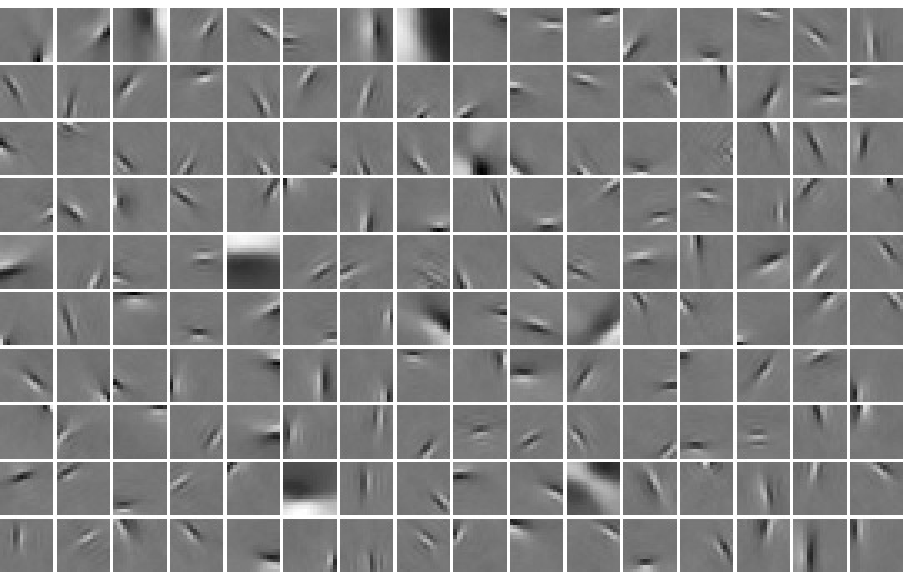
\includegraphics[width=0.5\linewidth]{fig1905}
      \caption{The ICA basis vectors of natural image
        patches.  \label{fig:ica_basis}}
    \end{figure}
    \begin{figure}[h]
      \centering
      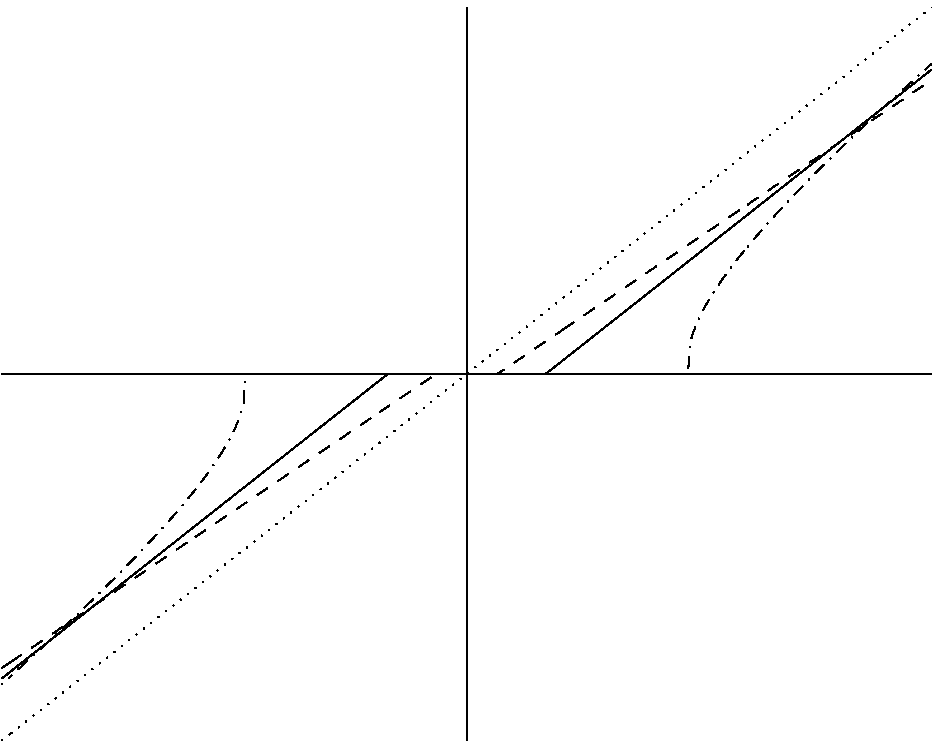
\includegraphics[width=0.5\linewidth]{fig1401}
      \caption{Different shrinkage functions. \label{fig:shrinkage}}
    \end{figure}
    \begin{figure}[h]
      \centering
      \subfloat[][Original]{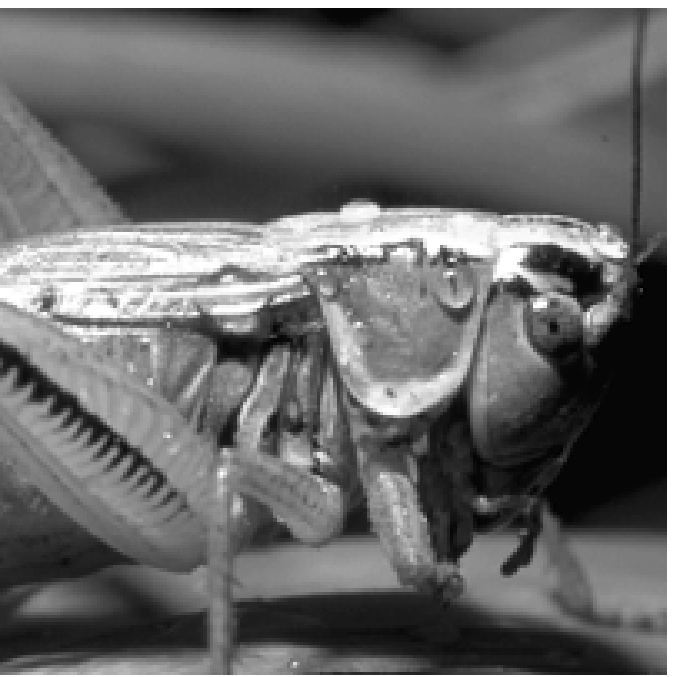
\includegraphics[width=0.45\linewidth]{fig1907a}}
      \hfill
      \subfloat[][Noisy]{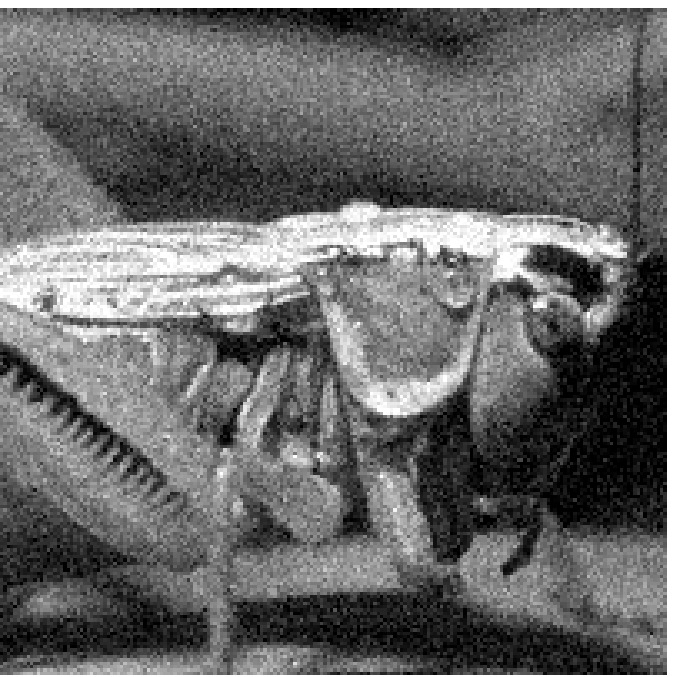
\includegraphics[width=0.45\linewidth]{fig1907b}}
      \\
      \subfloat[][Wiener filter
      denoising]{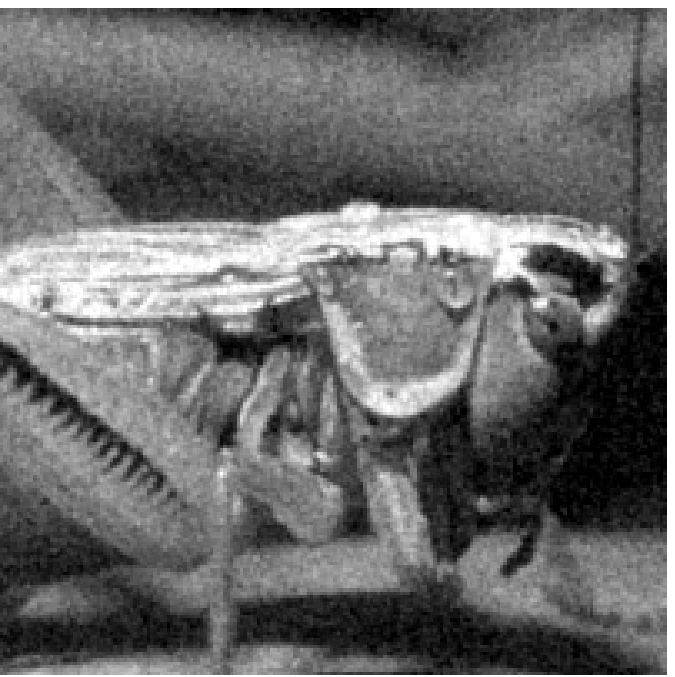
\includegraphics[width=0.45\linewidth]{fig1907c}}
      \hfill \subfloat[][ICA
      denoising]{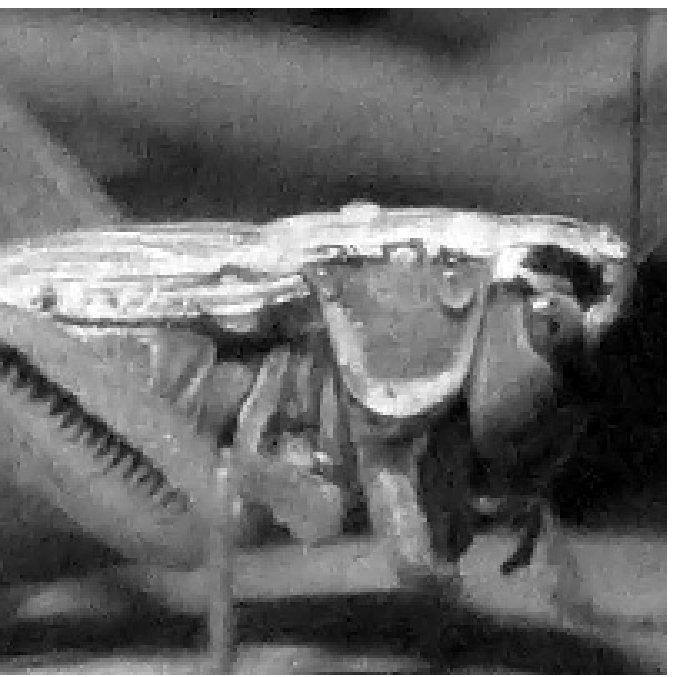
\includegraphics[width=0.45\linewidth]{fig1907d}}
      \caption{Image denoising experiment.  \label{fig:results}}
    \end{figure}
    
    
    % Reducing noise in natural images:

    % Collect the input vectors ${\bf x}$ from randomly chosen windows in the
    % image.

    % Assume a noise model:
    % \begin{displaymath}
    %   {\bf z} = {\bf x} + \mathbf{n} \; ,
    % \end{displaymath}
    % where the noise $\mathbf{n}$ is Gaussian and the ``signal'' ${\bf x}$ is
    % non-Gaussian.

    % Transform the data with a matrix ${\bf W}$ that is estimated with a variant 
    % of the FastICA algorithm:
    % \begin{displaymath}
    %   {\bf Wz} = {\bf Wx} + {\bf Wn} = {\bf s} + {\bf Wn}
    % \end{displaymath}

    % The noise ${\bf Wn}$ is still Gaussian whereas ${\bf s}$ becomes
    % super-Gaussian for suitable ${\bf W}$ (note: heavy tails!)

    % Cutting small values then removes mainly noise.

    % Finally: Transform back with ${\bf W}^T$ (note: ${\bf W}$ was orthogonal)

    % Is this somewhere?
    %\includepdf{ex9_answer_page4}
  \end{solution}

  

\end{enumerate}
\end{document}             % End of document.

%%% Local Variables: 
%%% mode: latex
%%% TeX-master: "ex09_solutions"
%%% End: 
